\subsubsection{External interfaces}

\begin{figure}[h]
	\centering
	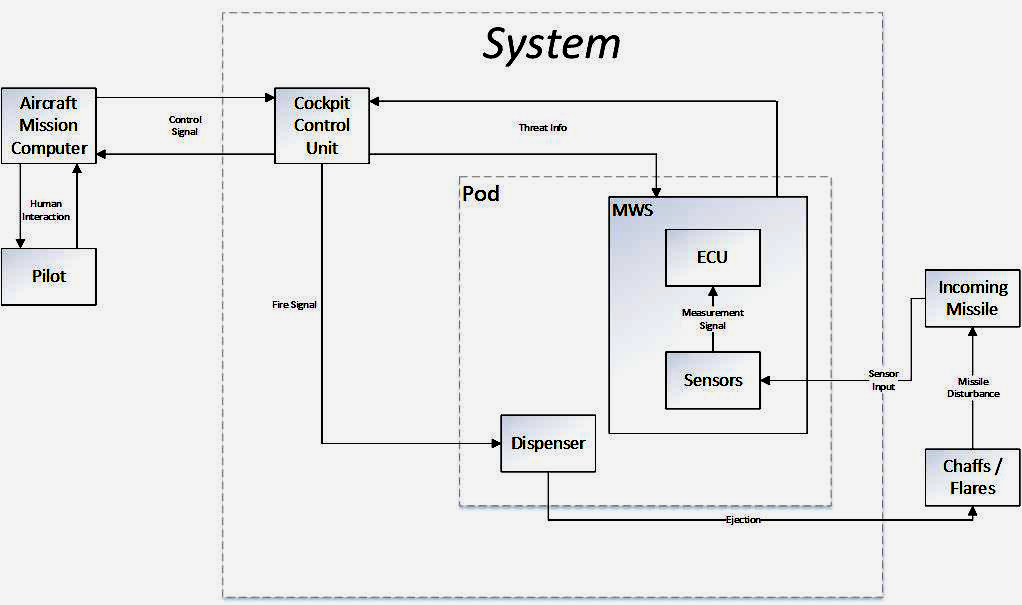
\includegraphics[scale=0.5]{./images/SignalFlowDiagram}\\
	\caption{Signal Flow Diagram}
    \label{fig:sigFlowDiagram}
\end{figure}
\begin{itemize}
\item {Interface identification and diagrams.}\\
blaa
\item {Project-unique identifier of interface}\\
blaa
\end{itemize}

\subsubsection{Internal interfaces}
This section describes the internal interfaces. The system interfaces can be seen on figure \ref{fig:sigOverviewIdentification}. The internal interfaces are:

\begin{itemize}
\item I-IF-MWSCTRL
\item I-IF-DISCTRL
\item I-IF-PODPWR
\end{itemize}

\paragraph{I-IF-MWSCTRL}

\begin{center}
\begin{tabular}{ | p{2cm} | l | p{2.3cm} | p{2.3cm} | l | p{1cm} |}
\hline
 \textbf{Interface name} & \textbf{Identification} & \textbf{Endpoint A} & \textbf{Endpoint B} & \textbf{Standard}\\ \hline

 MWS Control & I-IF-MWSCTRL & Cockpit unit & MWS & MIL-STD-1553-B\\ \hline

\end{tabular}
\end{center}

Some description...
\\
The data 
\begin{itemize}
\item Threat data (MWS $\rightarrow$ Cockpit unit)
	\begin{itemize}
	\item Direction relative to north
	\item Size
	\item Velocity
	\end{itemize}
\item Aircraft navigation data (Cockpit unit $\rightarrow$ MWS)
	\begin{itemize}
	\item Altitude
	\item Heading
	\item Position data
	\end{itemize}
\end{itemize}
The physical layer is defined by the MIL-STD-1553-B standard.


\paragraph{I-IF-DISCTRL}

\begin{center}
\begin{tabular}{ | p{2cm} | l | p{2.3cm} | p{2.3cm} | l | p{1cm} |}
\hline
 \textbf{Interface name} & \textbf{Identification} & \textbf{Endpoint A} & \textbf{Endpoint B} & \textbf{Standard}\\ \hline

 Dispenser Control & IF-DISCTRL & Cockpit unit & Dispenser assembly & MIL-STD-1553-B\\ \hline
 
\end{tabular}
\end{center}

Some description...\\
Something about data:
\begin{itemize}
\item direction to fire
\item what to fire (chaffs/flares)
\item pattern to fire
\item fire command
\end{itemize}

The physical layer is defined by the MIL-STD-1553-B standard.

\paragraph{I-IF-PODPWR}

\begin{center}
\begin{tabular}{ | p{2cm} | l | p{2.3cm} | p{2.3cm} | l | p{1cm} |}
\hline
 \textbf{Interface name} & \textbf{Identification} & \textbf{Endpoint A} & \textbf{Endpoint B} & \textbf{Standard}\\ \hline

 Pod power control & IF-PODPWR & Cockpit unit & Dispenser assembly and MWS & N/A\\ \hline
 
\end{tabular}
\end{center}

This analog signal connects from the cockpit unit to the dispenser assembly and the MWS in the pod. When asserted, this signal enables power to the dispenser assembly and MWS. When not asserted, the power is off.